\documentclass[12pt, a4paper, twoside]{article}
%todo make font size 11pt and make graphs bigger.

\usepackage{fontspec}
\usepackage{blindtext}
\usepackage{geometry}
\usepackage{setspace}
\usepackage{titlesec}
\usepackage{indentfirst}
\usepackage{graphicx}
\usepackage[italian]{babel}
\usepackage{catchfile} % used in \getenv command
\usepackage{multicol}
\usepackage{amsmath}
\usepackage{subcaption}
\usepackage[hang, flushmargin, multiple, bottom]{footmisc}
\usepackage{float}
\usepackage{array}
\usepackage{booktabs}
\usepackage{url}

\raggedbottom

%\setmainfont{Carlito}
\titlespacing*{\section}{0px}{3mm}{1mm}
\titlespacing*{\subsection}{0px}{3mm}{1mm}
\geometry{
  left=2cm,
  right=2cm,
  top=2cm,
  bottom=2cm
}
\setlength{\parindent}{10mm}
\graphicspath{ {./assets}, {../../assets} }

% Allow use of command \getenv{VARNAME}.
% Taken from: https://tex.stackexchange.com/questions/62010/can-i-access-system-environment-variables-from-latex-for-instance-home
\newcommand{\getenv}[2][]{
  \CatchFileEdef{\temp}{"|kpsewhich --var-value #2"}{\endlinechar=-1}%
  \if\relax\detokenize{#1}\relax\temp\else\let#1\temp\fi}

\begin{document}


\begin{center}
  \huge Misura dell'angolo di Brewster di un prisma mediante le formule di Fresnel \\
  \large Francesco Platini \getenv{MAT1}. Matteo Bonacini \getenv{MAT2}.\\ % see readme on how to use this
  \today
\end{center}

\begin{abstract}\label{sec:abstract}
In questo esperimento abbiamo analizzato il comportamento di un raggio di luce
che colpisce la superficie di un prisma di materiale ignoto.
Abbiamo verificato che l’intensità luminosa riflessa segua l’andamento
previsto dalle equazioni di Fresnel e abbiamo misurato il valore dell'angolo di Brewster
per il prisma.
I risultati ottenuti sono ?????????? compatibili/incompatibili % todo
\endinput

\end{abstract}

\section{Introduzione}\label{sec:introduzione}
Quando un raggio luminoso colpisce una superficie di separazione tra due
dielettrici con indici di rifrazione $n_1$ e $n_2$ diversi, si possono verificare
i fenomeni della riflessione e rifrazione.
Le equazioni di Fresnel, derivabili direttamente dalle equazioni di Maxwell, % fixme in equazioni ci va maiuscola?
descrivono un aspetto di questo comportamento, prevedendo quale frazione d'intensità
luminosa viene riflessa e quale rifratta per ciascuna delle due componenti di
polarizzazione.
Indichiamo con $R_\pi$ e $R_\sigma$ le frazioni d'intensità luminosa riflessa
polarizzate, rispettivamente, parallelamente e perpendicolarmente al piano
d'incidenza.
Si dimostra che valgono:

\begin{equation}
  R_\pi = \frac {
    n_2 \cos{\theta_i} - n_1 \cos{\theta_t}
  } {
    n_2” \cos{\theta_i} + n_1 \cos{\theta_t}
  }\label{eq:fresnel-eq-p}
\end{equation}

\begin{equation}
  R_\sigma = \frac {
    n_1 \cos{\theta_i} - n_2 \cos{\theta_t}
  } {
    n_1” \cos{\theta_i} + n_2 \cos{\theta_t}
  }\label{eq:fresnel-eq-s}
\end{equation}

\vspace{10mm}
\noindent dove $n_1$ e $n_2$ sono gli indici di rifrazione dei due mezzi, $\theta_i$ e
$\theta_r$ sono gli angoli d'incidenza e rifrazione del raggio luminoso.
Una dimostrazione rigorosa di come si ricavino \eqref{eq:fresnel-eq-p} e \eqref{eq:fresnel-eq-s} non è oggetto
di questo testo;
si veda Mazzoldi\cite{mazzoldi98} per ulteriori approfondimenti.

Variando $\theta_i$ e misurando l’intensità del raggio riflesso,
ci aspettiamo di osservare l'andamento previsto da \eqref{eq:fresnel-eq-p} e \eqref{eq:fresnel-eq-s} (a meno di una
costante moltiplicativa).
Il valore di $\theta_t$ viene ricavato dalla legge di Snell per la rifrazione:

\begin{equation}
  \frac {\sin{\theta_i}} {\sin{\theta_t}} = \frac {n_2} {n_1}
  \label{eq:legge-snell}
\end{equation}

\noindent Le formule prevedono che $R_\pi$ si annulli per un certo valore di $\theta_i$,
che indicheremo con $\theta_B$.
Questo angolo prende il nome di Angolo di Brewster, ed è previsto dalla legge di Brewster:

\begin{equation}
  \theta_B = \arctan{
    \frac {n_2} {n_1}as
  }\label{eq:legge-brewster}
\end{equation}

\noindent  L’angolo di Brewster gode di alcune proprietà utili in diverse applicazioni
sperimentali.
Per approfondimenti, si consulti Mazzoldi\cite{mazzoldi98}.
\endinput


\section{Apparato sperimentale e svolgimento}\label{sec:apparato-sperimentale-e-svolgimento}
\subsection{Apparato sperimentale}\label{subsec:apparato-sperimentale}
  L’apparato sperimentale è riportato in Fig.\ref{fig:apparato-strumentale}.
  Un prisma(\rom{5}) di vetro di indice di rifrazione $n_2$ sconosciuto, montato su un servomotore \emph{SM-S2309S}\footnote{http://descargas.cetronic.es/microservo.pdf},
  è posizionato al centro di una guida circolare graduata(\rom{4}).
  Un laser(\rom{1}) a luce rossa e due filtri polaroid(\rom{2}, \rom{3}) sono
  allineati con il prisma. Un sensore di intensità luminosa(\rom{6}) \emph{TEMT6000}\footnote{https://www.sparkfun.com/datasheets/Sensors/Imaging/TEMT6000.pdf},
  collegato ad un microcontrollore(\rom{7}) \emph{Arduino Uno (ATmega328)}\footnote{http://store.arduino.cc/products/arduino-uno-rev3}%
  \footnote{Da qui in avanti, si userà il nome abbreviato \emph{Arduino} al posto di \emph{Arduino Uno} per riferirsi al microcontrollore.},
  è libero di ruotare lungo la guida.
  Il circuito che collega \emph{Arduino} e sensore è schematizzato in Fig.\ref{fig:diagramma-circuito}.
  %
  Il servomotore permette di ruotare il prisma con una risoluzione angolare di ${1.0^\circ \pm 0.5^\circ}$.
  L'apparato Arduino-sensore fornisce una misura dell'intensità luminosa presente
  sulla superficie del sensore nell'intervallo $I = [0, 1000]$ unità arbitrarie,
  con un'incertezza sistematica massima di $0.8\%$ (si rimanda a Sez.\ref{subsec:calcolo-incertezza-strumentale}
  per la dimostrazione di come è stato ottenuto questo valore).
%
  \begin{figure}[h]
    \centering
    \begin{subfigure}{.47\textwidth}
      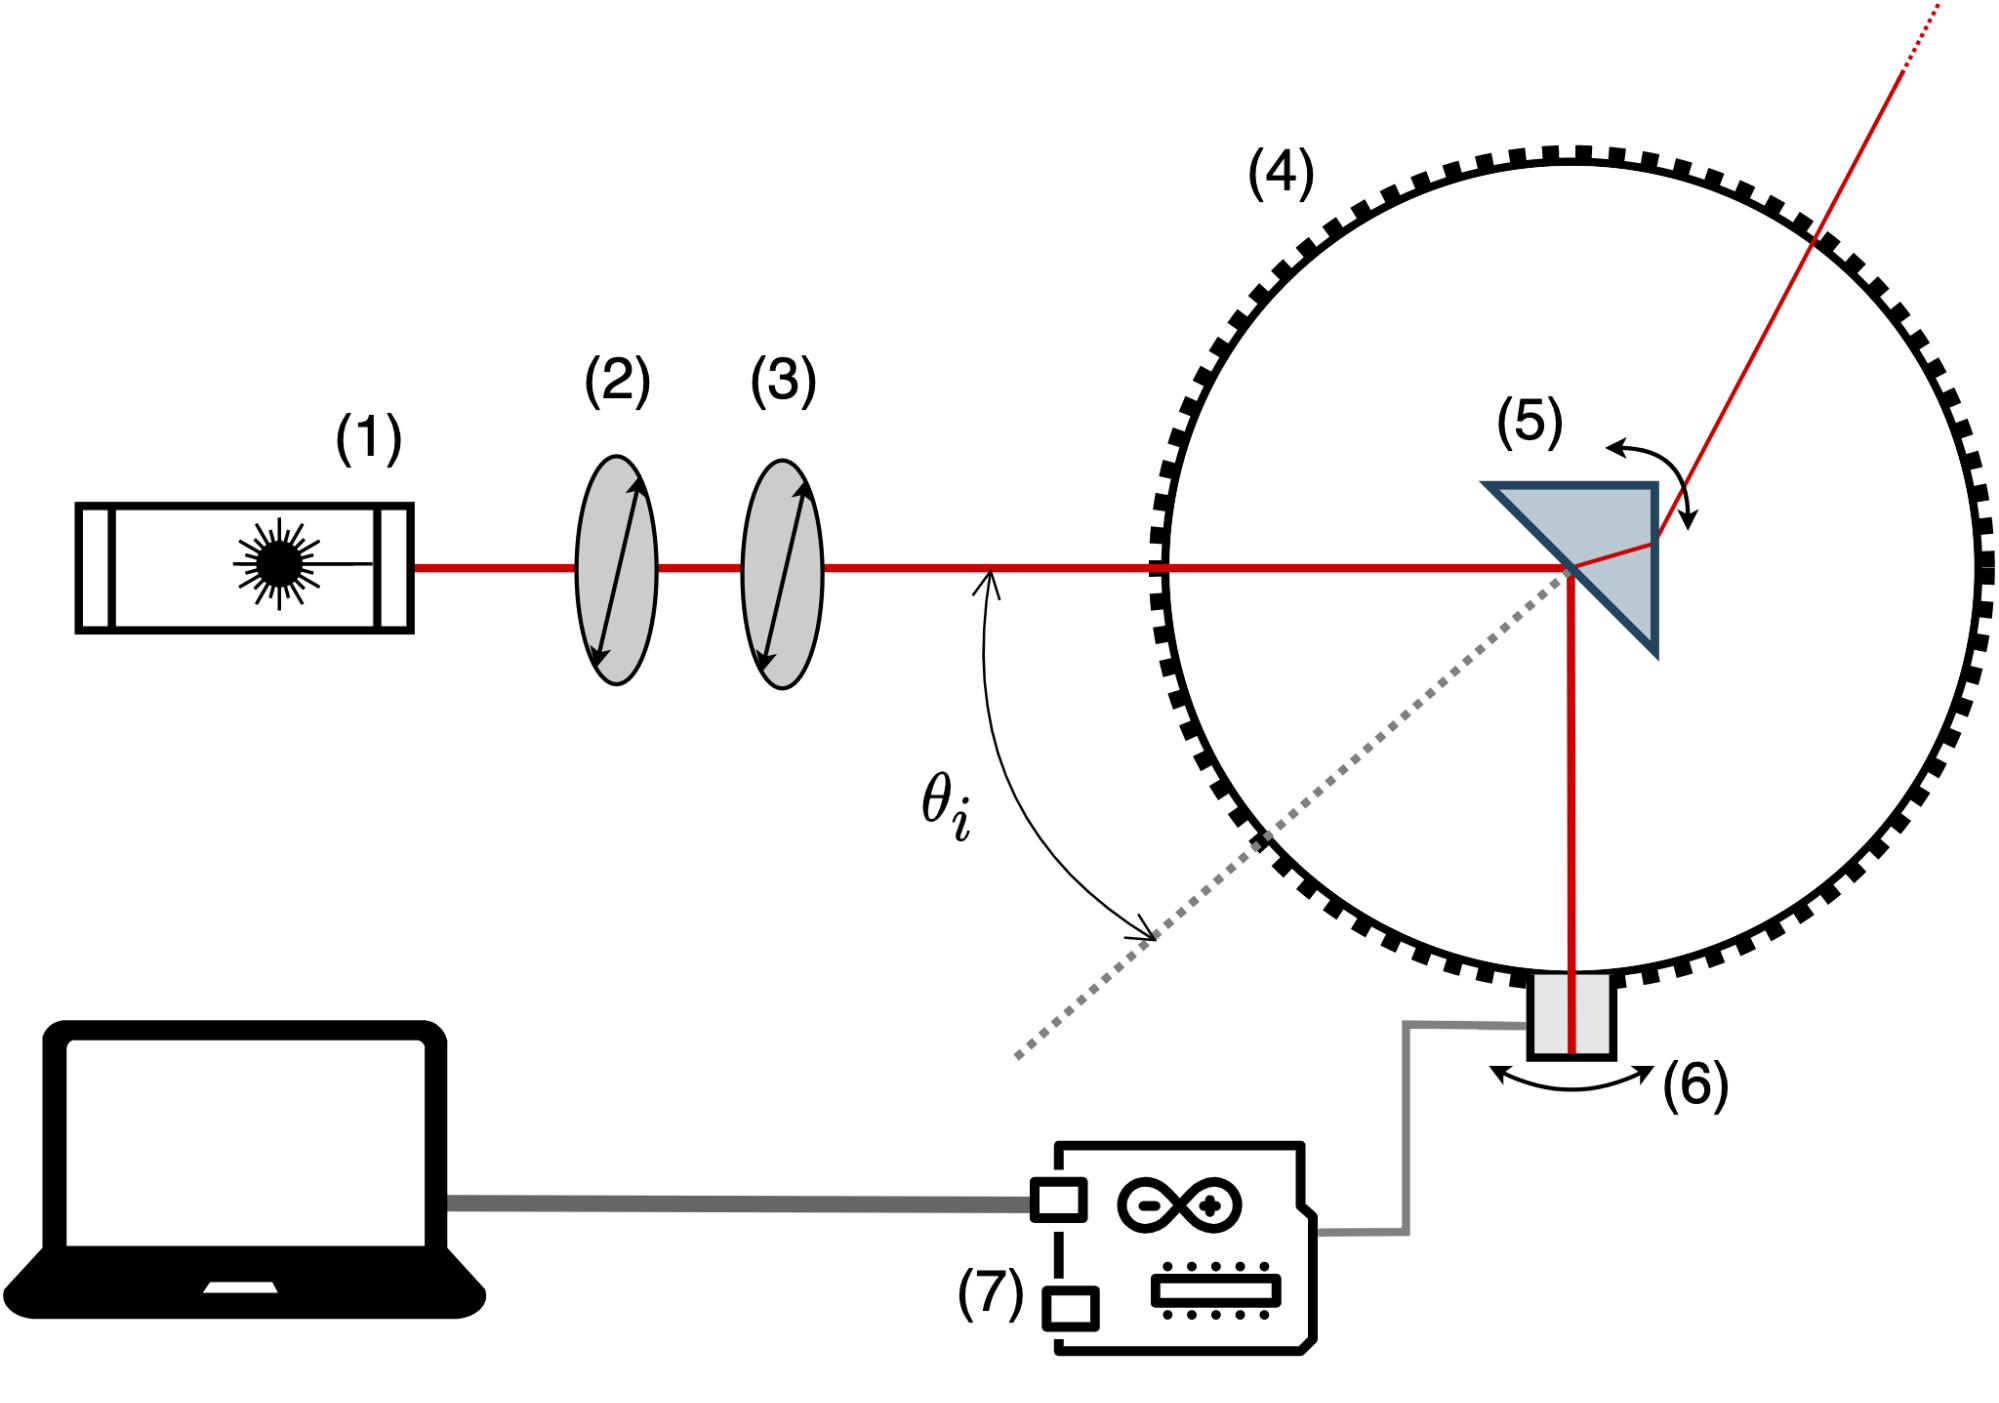
\includegraphics[width=8cm]{instrumental-apparatus.png}
      \caption{
        \emph{
          Apparato sperimentale. A partire da sinistra, in senso orario,
          si trovano: laser(\rom{1}), filtri polaroid(\rom{2}, \rom{3}), guida circolare(\rom{4}),
          prisma(\rom{5}), sensore(\rom{6}), Arduino(\rom{7}). Il servomotore non è riportato.
        }
      }
      \label{fig:apparato-strumentale}
    \end{subfigure}%
    \hspace{5mm}
    \begin{subfigure}{.47\textwidth}
      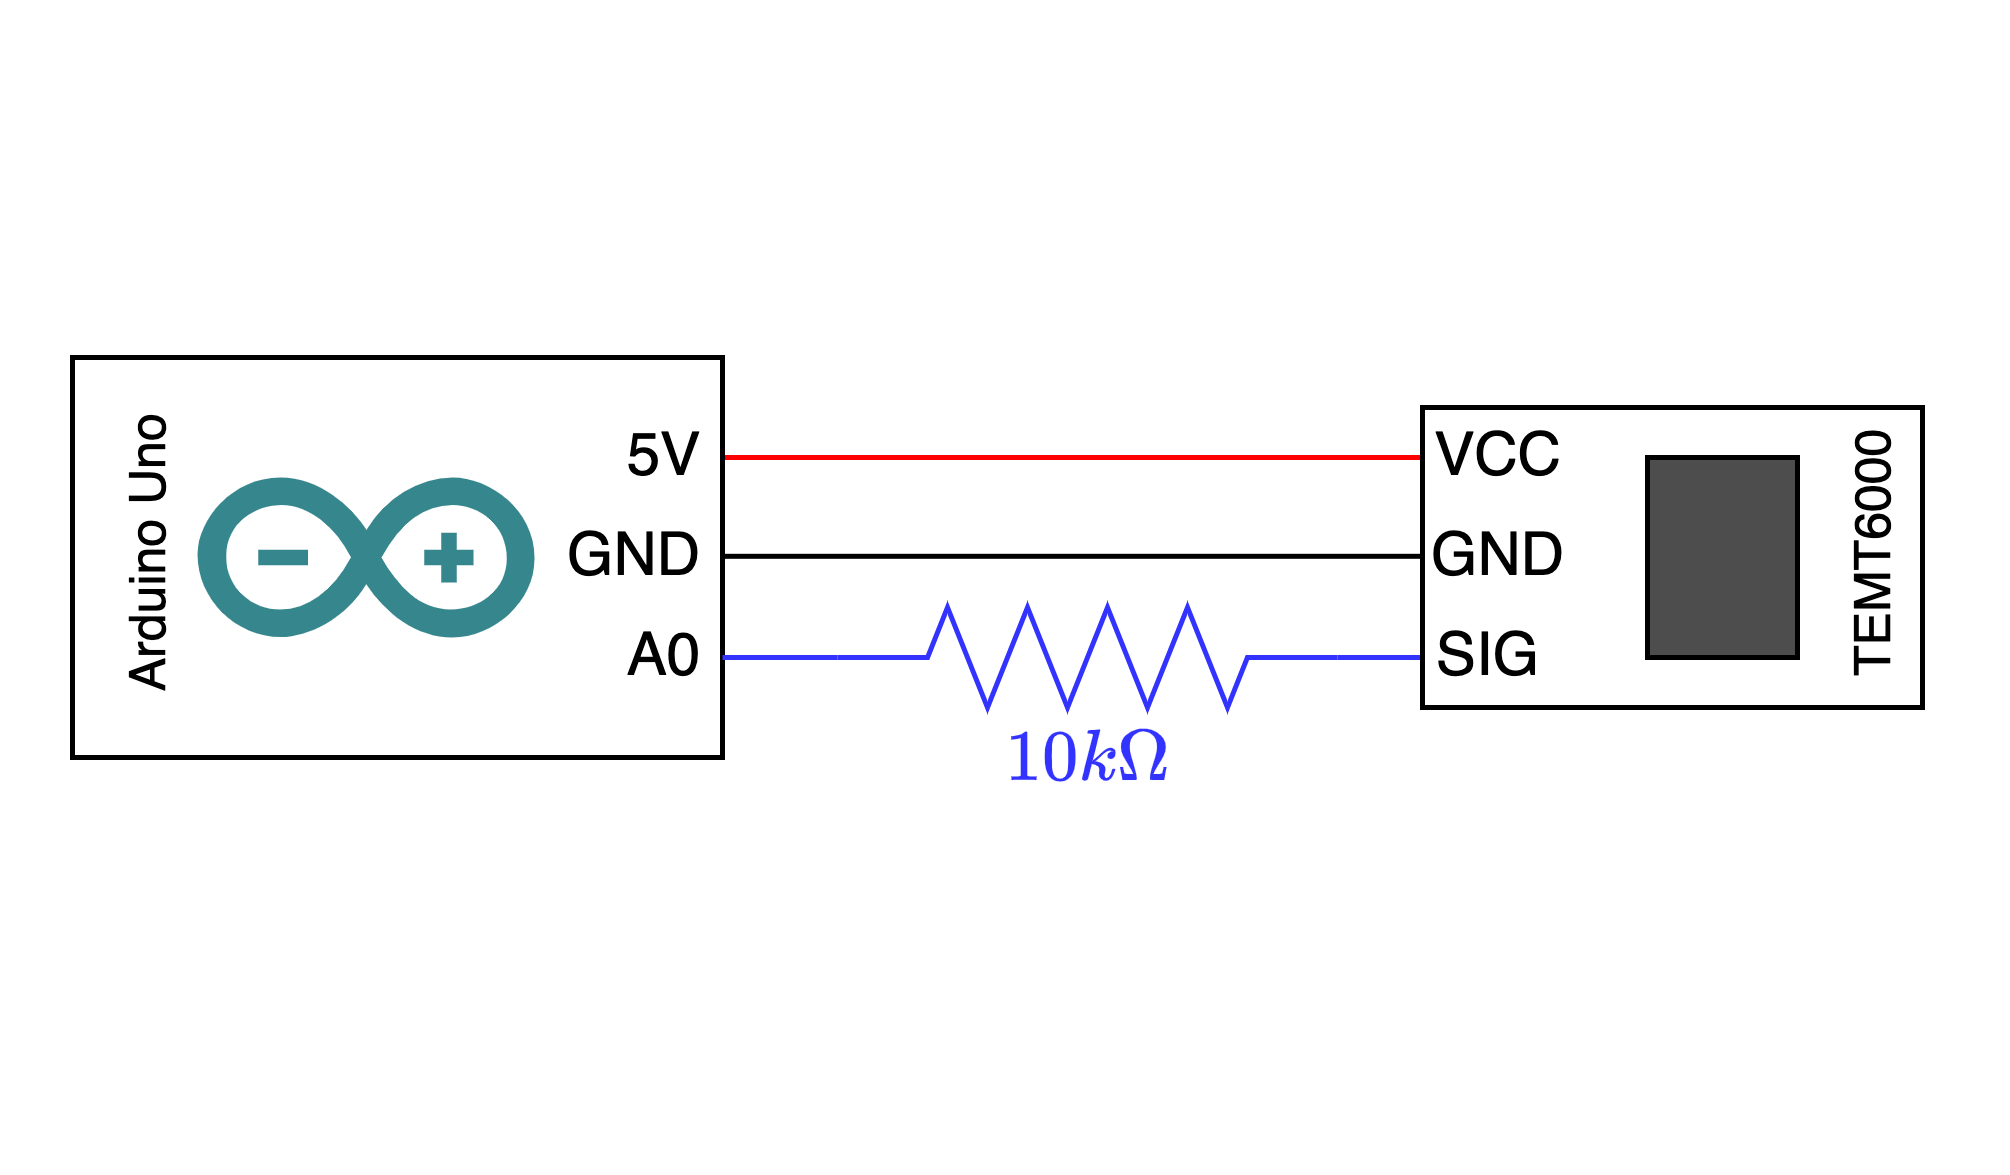
\includegraphics[width=8cm]{circuit-diagram.png}
      \caption{
        \emph{
          Schema circuitale. I pin $\text{VCC}$ e $\text{GND}$ del sensore sono collegati
          all'alimentazione di Arduino. Il pin $\text{SIG}$
          del sensore è collegato ad un input analogico di Arduino, tramite una
          resistenza da $10k\Omega$.
        }
      }
      \label{fig:diagramma-circuito}
    \end{subfigure}
    \caption{\emph{Apparato sperimentale e schema circuitale.}}
  \end{figure}
%
\subsection{Procedura sperimentale}\label{subsec:procedura-sperimentale}
  Abbiamo seguito la procedura sperimentale riportata di seguito, ripetuta due
  volte: una per raccogliere i dati relativi a $R_\pi$ e una per i dati relativi
  a $R_\sigma$. Questa procedura è stata adattata da quanto descritto in Lipson\cite{lipson20}.
  \begin{enumerate}
    \item%
      Abbiamo posizionato il polaroid(\rom{3}) in modo che la polarizzazione del
      fascio laser fosse parallela al lato del prisma, e abbiamo aggiustato l'angolo
      del laser rispetto ad esso, in modo da evitare che il fascio
      polarizzato uscente dal laser venisse bloccato.
    \item%
      Abbiamo posizionato il sensore e il prisma in modo da rendere
      massimo l'angolo $\theta_i$, con il vincolo che
      tutto il fascio laser fosse contenuto sulla superficie del prisma\footnote{Per $\theta_i \to 90^\circ$, la
      proiezione del fascio laser sul prisma è un'ellisse di semiasse maggiore $a \to +\infty$. Chiaramente, non appena
      $a$ supera la lunghezza del lato del prisma, le equazioni \eqref{eq:fresnel-eq-p} e \eqref{eq:fresnel-eq-s} perdono
      la loro validità.}.
    \item%
      Ruotando il polaroid(\rom{2}), abbiamo ridotto l’intensità del fascio laser
      incidente sul prisma, fino a che Arduino non ha potuto rilevare una
      variazione significativa del segnale del sensore.
      Questo ci ha permesso di sfruttare l'intero intervallo di operatività del convertitore analogico-digitale di Arduino.
    \item%
      Abbiamo acquisito l'intensità luminosa rilevata dal sensore in questo punto,
      poi abbiamo ruotato il prisma in senso orario e abbiamo
      allineato il sensore di conseguenza.
    \item%
      Abbiamo ripetuto il passo precedente fino a raggiungere un valore di $\theta_i$
      il più possibile vicino a zero.
    \item%
      Abbiamo ruotato di $90^\circ$ il polaroid(\rom{3}) e ripetuto l'intera
      procedura un'altra volta.
  \end{enumerate}
  %
  I dati che abbiamo raccolto in questo modo \emph{non} sono
  i coefficienti $R_\pi$ e $R_\sigma$, ma differiscono da essi per una costante
  moltiplicativa $I_0$; questa verrà determinata tramite un \emph{fit}\footnote{Avremmo potuto misurare
  questo valore direttamente, ma così facendo avremmo dovuto
  abbassare ulteriormente l'intensità del fascio laser e non avremmo più potuto
  sfruttare l'intero intervallo di operatività di Arduino.}, come descritto in Sez.$\ref{subsec:analisi-coefficienti}$.
\endinput



\section{Risultati e discussione}\label{sec:risultati-e-discussione}
  I risultati ottenuti sono riassunti in Fig.\ref{fig:dati-raw}.
  I parametri risultanti dal \emph{fit} sono riassunti in Tab.\ref{tab:risultati-fit}.
  I fit sono stati svolti usando l'algoritmo \emph{Gradient}\footnote{https://reference.wolfram.com/language/ref/NonlinearModelFit.html} di \emph{Woflram Mathematica}\footnote{https://www.wolfram.com/mathematica/}, e le rispettive incertezze %todo add ref
  sono date dagli errori standard dei parametri ottenuti dal \emph{fit}.                                          %todo add ref
  Qualitativamente, l'andamento è concorde con quanto atteso. In Fig.\ref{fig:raw-pi}
  si vede chiaramente che la funzione raggiunge lo zero per un certo angolo $\theta$,
  mentre in Fig.\ref{fig:raw-sigma} la funzione cresce monotonamente.
  %\footnote{In realtà nella nostra implementazione il valore di $V_{sig}$ è
  %  moltiplicato per una costante $k = (1024 \cdot 5)^{-1 V^{-1}}$, in modo
  %  da ottenere un intervallo di valori in uscita compreso in un range tra $0$ e
  %  $1000$.}
  \begin{figure}[H]
    \centering
    \caption{Dati raccolti}
    \begin{subfigure}[t]{.4\textwidth}
      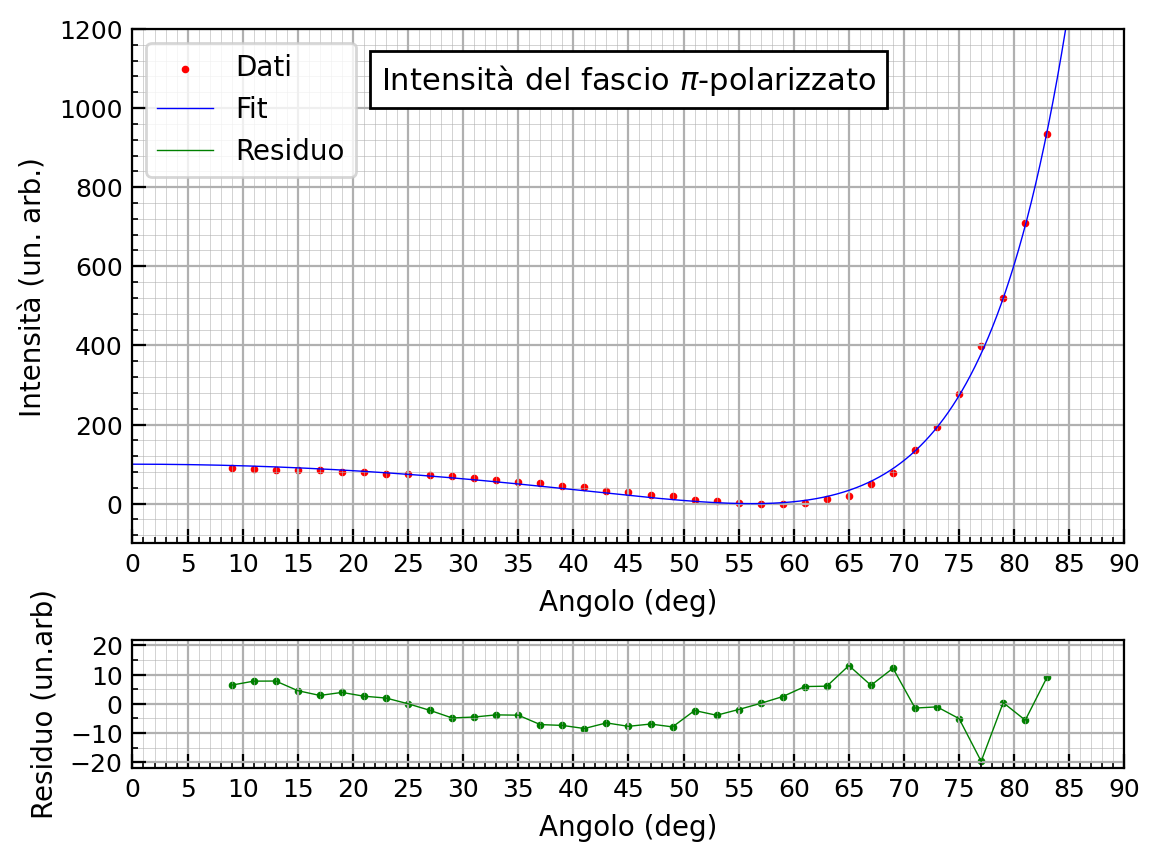
\includegraphics[width=7cm]{./graphs/raw-pi.png}
      \caption{
        \emph{
          Dati di intensità luminosa con luce polarizzata perpendicolarmente al
          piano di incidenza e relativo fit. Dal grafico si vede chiaramente che
          l'intensità luminosa si annulla per un certo valore di $\theta_i$.
        }
      }
      \label{fig:raw-pi}
    \end{subfigure}
    %
    \hspace{20mm}
    %
    \begin{subfigure}[t]{.4\textwidth}
      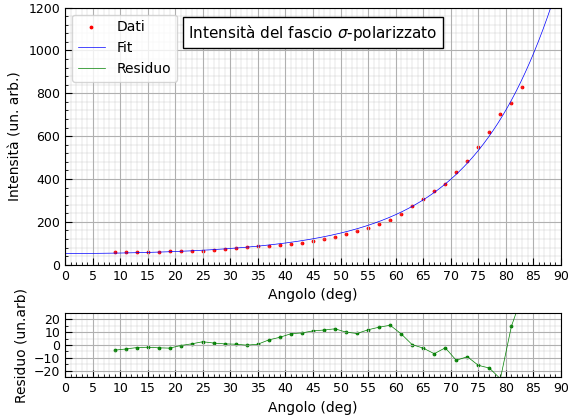
\includegraphics[width=7cm]{./graphs/raw-sigma.png}
      \caption{
        \emph{
          Dati di intensità luminosa con luce polarizzata parallelamente al
          piano di incidenza e relativo fit.
        }
      }
      \label{fig:raw-sigma}
    \end{subfigure}
    \label{fig:dati-raw}
  \end{figure}
  %
  \begin{table}[ht]
    \centering
    \caption{
      Risultati dei \emph{fit} dei dati raccolti. Le intensità sono espresse in unità arbitrare, gli indici
      di rifrazione e i chi quadro ridotti sono numeri puri.
    }
    \begin{tabular}[t]{cc}
      \toprule
      Parametro &Valore ottenuto\\
      \midrule
      $I_{0\pi}$ &$2550 \pm 10 (u. a.)$ \\
      $I_{0\sigma}$ &$1350 \pm 20 (u. a.)$ \\
      $n_{2\pi}$ &$1.493 \pm 0.006$    \\
      $n_{2\sigma}$ &$1.490 \pm 0.010$    \\
      $\tilde \chi^2_\pi$ &$0.71$ \\
      $\tilde \chi^2_\sigma$ &$1.17$ \\
      \bottomrule
    \end{tabular}\label{tab:risultati-fit}
  \end{table}
  %
  Abbiamo misurato valori nell'intervallo di ${\theta_{min} \leq \theta \leq \theta_{max}}$,
  con ${\theta_{min} = 7^\circ \pm 0.5^\circ}$ e $\theta_{max} = 83^\circ \pm 0.5^\circ$.
  Le dimensioni del lato del prisma utilizzato ($15mm$ di lunghezza) non permettevano
  di andare oltre $\theta_{max}$ senza che il fascio venisse alterato, mentre il
  limite di $\theta_{min}$ ci è stato imposto dalla geometria del sensore.
  Abbiamo scelto un passo angolare di $2^\circ$ per permetterci di prendere un
  numero adeguato di misure, senza allungare eccessivamente la durata dell'esperimento.
  Il campione di dati riportato in Fig.\ref{fig:dati-raw} è quello che segue meglio
  l'andamento previsto.
  Le incertezze associate ad ogni punto sono state ottenute come somma somma di
  incertezze sistematiche dovute all'attrezzatura e di incertezze casuali, come
  descritto in Sez.\ref{subsec:calcolo-incertezza-strumentale} e Sez.\ref{subsec:calcolo-incertezza-casuale}.

  Normalizzando i dati, si ottengono i risultati mostrati in Fig.\ref{fig:normalised-coefficients} %todo capire se per normalizzare basta dividere per I_0, o se conviene imporre anche che i due n2 siano uguali.
                                                                    %  ceh in realtà ci sta prenderne la media per soddisfare a condizione di Lipson.
  assieme all'andamento previsto\footnote{Calcolato supponendo di avere un valore di $n_2 = 1.519$, %todo expand me
  caratteristico per il vetro K9 alla lunghezza della luce rossa.}.
  %
  \begin{figure}[H]
    \centering
    \caption{Smegma}
    \begin{subfigure}{.4\textwidth}
      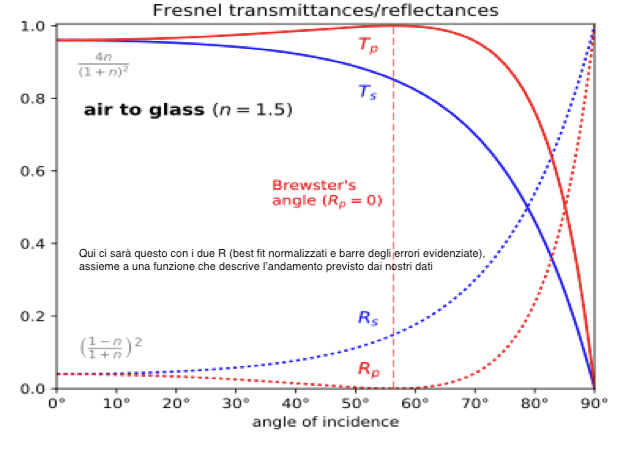
\includegraphics[width=7cm]{./graphs/normalised-coefficients.png}
      \caption{
        \emph{
          spregna
        }
      }
      \label{fig:normalised-coefficients}
    \end{subfigure}%
    \hspace{20mm}
    \begin{subfigure}{.4\textwidth}
      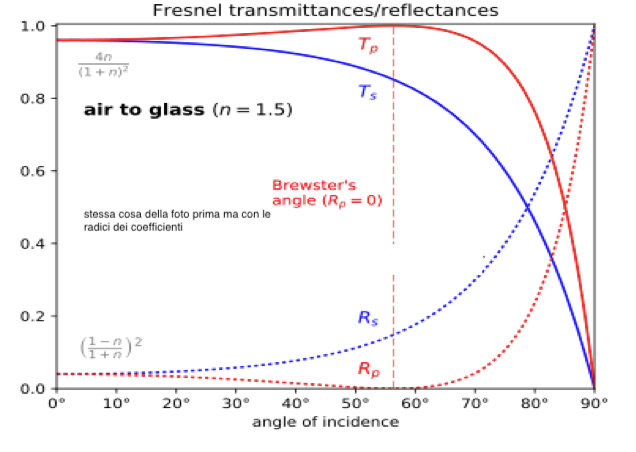
\includegraphics[width=7cm]{./graphs/amplitude-coefficients.png}
      \caption{
        \emph{
          bora
        }
      }
      \label{fig:coefficienti-ampiezza}
    \end{subfigure}
  \end{figure}
%
\subsection{Misura dell'angolo di Brewster}\label{subsec:angolo-di-brewster}
  Inserendo nell'equazione \eqref{legge-brewster} $n_1 = 1.000$ e $n_2 = 1.492 \pm 0.008$
  otteniamo un valore per l'angolo di Brewster $\theta_B = \arctan{(n_2 / n_1)} = \arctan{(1.492)} = 56.2^\circ \pm 0.1^\circ$. Il valore di $n_2$ utilizzato è la media
  dei due coefficienti in Tab.\ref{tab:risultati-fit} e l'incertezza associata è data dalla formula generale per la
  propagazione degli errori (come descritto in Taylor\cite{taylor99}).
  Possiamo ottenere un'altra stima per $\theta_B$ con un \emph{fit} parabolico nella stretta regione
  dove $R_\pi$ si annulla; il vertice della parabola è la miglior stima per $\theta_B$.
  La funzione uitlizzata per il \emph{fit} è $y = a(x - \theta_B)^2$, dove il parametro $\theta_B$ è la
  miglior stima per il valore dell'angolo di Brewster.
  Il risultato ottenuto è mostrato in figura \ref{fig:brewsters-angle}. I valori numerici
  dei parametri risultanti dal fit sono riportati in Tab.\ref{fit-brewster}
  %
  \begin{figure}[h]
    \centering
    \caption{brema}
    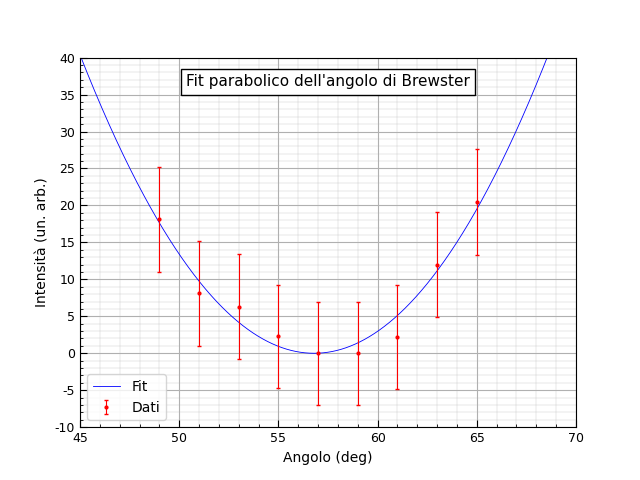
\includegraphics[width=7cm]{./graphs/brewsters-angle.png}
    \label{fig:brewsters-angle}
  \end{figure}
  \begin{table}[ht]
    \centering
    \caption{
      Risultati numerici del \emph{fit} parabolico per determinare l'angolo di Brewster.
    }
    \begin{tabular}[t]{cc}
      \toprule
      Parametro &Valore ottenuto\\
      \midrule
      $a$ &$0.29 \pm 0.02 (u.a.)$ \\
      $\theta_B$ &$56.8^\circ \pm 0.2^\circ$ \\
      \bottomrule
    \end{tabular}\label{tab:fit-brewster}
  \end{table}
  % TODO
\endinput





\section{Conclusioni}\label{sec:conclusioni}
Per quanto riguarda la prima parte dell'esperimento, i dati raccolti seguono l'andamento
previsto. Il \emph{fit} ottenuto è soddisfacente, e
il valore ottenuto per $n_2$ è compatibile con il coefficiente di rifrazione del
vetro $n = 1.5$.
È possibile che ci sia stata una sovrastima delle incertezze, visto il valore di
$\tilde \chi^2_\pi < 1$, ma questa ipotesi è difficile da confermare con il numero
limitato di dati raccolti.
Riguardo alla seconda parte dell'esperimento, abbiamo ottenuto due stime di
$\theta_B$ in parziale disaccordo: $\theta_B = 56.2^\circ \pm 0.1^\circ$ e $\theta_B 56.8^\circ \pm 0.2^\circ$.
Tuttavia, l'indice di rifrazione tipico del vetro è compreso tra $n=1.50$ e $n=1.53$, e se
inseriamo questi valori nell'equazione \eqref{legge-brewster} osserviamo che i risultati
ottenuti rientrano nell'intervallo di valori attesi $56.3 < \theta_{B} < 56.8^\circ$.

Nello svolgere l'esperimento siamo stati fortemente limitati dal tempo a disposizione
e siamo confidenti che il nostro apparato sperimentale possa ottenere risultati ancora
più accurati se potessimo acquisire ulteriori set di dati. In ogni caso, consideriamo
questo esperimento un successo.
\endinput



\bibliographystyle{unsrt} % We choose the "plain" reference style
\bibliography{./docs/report/fresnelReportRefs.bib} % Entries are in the fresnelReportRefs.bib file

\newpage
\section{Appendice}\label{sec:appendice}
\subsection{Calcolo incertezza strumentale}\label{subsec:calcolo-incertezza-strumentale}
  Per effettuare le misure d'intensità luminosa, Arduino compara
  il segnale $V_{sig}$ in uscita dal sensore \emph{TEMT6000} con il potenziale
  $V_{cc}$ dell'alimentatore.
  Dato che il segnale $V_{cc}$ può essere soggetto a fluttuazioni sistematiche significative\footnote{Basti pensare a un alimentatore che si riscalda durante la presa dati,
  causando un progressivo abbassamento di $V_{cc}$.}
  (dell'ordine del ~10\%)\footnote{Arduino può essere alimentato con potenziale compreso tra $\sim 4.5V$ e $\sim 5.5V$.}, abbiamo utilizzato il potenziale di riferimento
  $V_{ref}$ di \emph{Arduino}, mantenuto costante a $1.1V$, come strumento di
  calibrazione.
  Per ogni misurazione l'\emph{ADC} svolge un calcolo di questo tipo:
  %
  \begin{equation}
    V_i' = k * \frac {V_i} {V_{cc}}
    \label{eq:misura-adc}
  \end{equation}
  %
  \noindent dove $V_i'$ è il valore di misurato, $V_i$ è il valore vero e $k$
  è una costante di proporzionalità. Conoscendo il valore nominale
  di $V_{ref}$\footnote{Trascuriamo il valore iniziale di \emph{offset}, visto che
  a noi importa solo della precisione della misura e non della sua accuratezza.}, possiamo rimuovere la
  dipendenza da $V_{cc}$. Per ogni misura $I_i$ di intensità, andiamo a misurare sia $V_{sig}$ che $V_{ref}$.
  I valori $V_{sig}'$ e $V_{ref}'$ che otteniamo sono dati dalla \eqref{eq:misura-adc}:
  %
  \vspace{-10mm}
  \begin{multicols}{2}
    \begin{equation}
      V_{ref}' = k * \frac {V_{ref}} {V_{cc}}
      \label{eq:vref-misura}
    \end{equation}
  \break
    \begin{equation}
      V_{sig}' = k * \frac {V_{sig}} {V_{cc}}
      \label{eq:vsig-misura}
    \end{equation}
  \end{multicols}
  %
  \noindent Dividendo la \eqref{eq:vsig-misura} per la \eqref{eq:vref-misura} troviamo il valore vero cercato $V_{sig}$.
  La formula finale è quindi (riportata con le incertezze già calcolate):
  %
  \begin{equation}
    V_{sig} = \frac {
      V_{ref} (\pm 0.4\%)
    } {
      V'_{ref} (\pm 0.2\%)
    } V'_{sig} (\pm 0.2\%)
    \label{eq:misura-intensità}
  \end{equation}
  %
  In questa formula compaiono due diverse sorgenti di errore:
  l'\emph{ADC} di \emph{ATmega328P} e il potenziale di riferimento $V_{ref}$
  di Arduino.
  % Questo magari va messo in una nota?
  %abbiamo considerato trascurabile l’incertezza strumentale del sensore, dato
  %che non è riportata nel \emph{datasheet} e
  %qualsiasi suo effetto sarà incluso
  %nelle incertezze casuali stimate in (vedi sezione 6.2).
  Abbiamo ottenuto l’incertezza dell’\emph{ADC} direttamente dal
  \emph{datasheet}\cite{atmega} di \emph{ATmega328P} (Sez.23.1):
  il produttore indica un'incertezza massima assoluta di $\pm 2LSB \approx 0.2\%$.
  Questo valore tiene conto di tutte le possibili fonti di errore interne
  all’\emph{ADC} ed è da considerarsi come limite superiore.
  Per quanto riguarda l'incertezza del potenziale di riferimento, abbiamo
  utilizzato il lavoro di Main\cite{main}, dove è stato misurato un errore sistematico
  massimo dello $0.4\%$.
  Propagando linearmente le incertezze nella formula \eqref{eq:misura-intensità} si ottiene un incertezza
  strumentale dello $0.8\%$.

\subsection{Calcolo incertezza casuale}\label{subsec:calcolo-incertezza-casuale}
  % Questa incertezza è data dall'allineamento del sensore.
  A causa di limitazioni strumentali, non ci è stato possibile ottenere un campione
  numeroso di misure per ogni angolo. Possiamo ottenere ugualmente
  una stima delle incertezze casuali assumendo che:
  1) le misure di intensità sono distribuite in modo normale attorno a un valore
    medio $\mu_i$, proprio di ogni angolo;
  2) tra un angolo e un altro la distribuzione differisce solo per la media e non per la
    deviazione standard $\sigma$.
  Queste sono giustificate dal fatto che il modo in cui vengono raccolti i dati
  non è dipendente dall'angolo a cui si trova il sensore.
  Abbiamo quindi stimato $\sigma$ tenendo in considerazione degli scarti quadratici
  dei campioni di ogni angolo.
  Abbiamo usato la formula:
  %
  \begin{equation}
    \sigma = \sqrt{
      \frac {
        \sum_{i = \theta_{min}}^{\theta_{max}} \left(
          \sum_{j = 0}^{N_i} (x_{ij} -\mu_i)^2
        \right)
      } {
        \nu
      }
    }
  \end{equation}
  %
  \noindent dove $N_i$ è il numero di dati nel campione $\vec{x}_i$.
  $\nu$ è il numero di gradi di libertà dei dati. La miglior stima per l'incertezza
  sull'intensità luminosa, infine, è data dalla variazione standard della media $\sigma^*$.
  Il risultato ottenuto è $\sigma^* = 7.30 (\text{unità arbitrarie})$.
                                                                      % noi interessano le fluttuazioni
                                                                      % statistiche, quindi questa roba non viene
                                                                      % divisa per sqrt(n). Se ci interessasse la
                                                                      % singola misura, dovremmo
                                                                      % dividere.
  % btw qui ci sarebbe da dividere per sqrt(2), visto che ho preso 2 punti per ogni angolo.
\endinput

% Continuo con la roba dell'errore. Arduino può misurare un errore di intensità
% per via di Vcc. Ora, vcc può avere variazioni rapide, ma può anche avere
% variaziuoni più lente, dell'ordine di tutto lo sweep di angoli, che sono
% in pratica erorri sistematici. Questo fixa tutto.



\end{document}

%In this document somasdmeters
%were added. There is an encoding package,
%and pagesize and fontsize parameters.

